\documentclass[11pt]{article}
\usepackage[margin=1in]{geometry}
\usepackage{amsmath,amssymb,amsthm,mathtools}
\usepackage{booktabs,longtable,array}
\usepackage{tikz}
\usetikzlibrary{decorations.pathreplacing,positioning,fit,calc}
\usepackage[hidelinks]{hyperref}
\usepackage[capitalise,nameinlink]{cleveref}

\newtheorem{theorem}{Theorem}
\newtheorem{lemma}[theorem]{Lemma}
\newtheorem{corollary}[theorem]{Corollary}
\newtheorem{proposition}[theorem]{Proposition}
\theoremstyle{definition}
\newtheorem{definition}[theorem]{Definition}
\newtheorem{remark}[theorem]{Remark}
\newtheorem{example}[theorem]{Example}
\crefname{lemma}{Lemma}{Lemmas}
\crefname{theorem}{Theorem}{Theorems}

\setcounter{MaxMatrixCols}{12}
\newcommand{\rev}{\operatorname{rev}}
\newcommand{\cG}{\mathcal{G}}
\newcommand{\steps}{\operatorname{steps}}
\newcommand{\inn}{\mathrm{in}}

\title{Longer Thomason chains via 3-pole composition}
\author{AUTHOR NAME(S)\thanks{AFFILIATION. Email: EMAIL.}}
\date{Draft, \today}

\begin{document}
\maketitle

\begin{abstract}
Thomason's lollipop algorithm turns Smith's theorem into a procedure: given a Hamiltonian cycle
of a cubic graph and one of its edges, it walks through a sequence of Hamiltonian paths and
stops at a second Hamiltonian cycle through that edge. The walk can be exponentially long. The
best known lower bound, due to Bria\'nski and Szady, is $\Omega(1.1812^n)$ steps on 3-connected
planar cubic graphs. We construct 3-connected planar cubic graphs with exactly three Hamiltonian
cycles on which the algorithm takes $\Theta(\rho^{n/6})$ steps, where
$\rho = 2.94771\ldots$ is the largest root of $\lambda^4-2\lambda^3-2\lambda^2-2\lambda-1$. Since
$\rho^{1/6} = 1.197422\ldots$, this is $\Omega(1.19742^n)$.

The construction comes from a general method for analysing the lollipop walk across 3-edge cuts.
We prove that, across a 3-edge cut, the walk either behaves exactly as in the graph with one
side contracted, or turns back (the \emph{Mirror Lemma}). The side of such a cut away from the
start acts as a finite automaton that does not depend on the rest of the graph (the
\emph{Transducer Theorem}).
For sides in which every pair of ports is joined by a unique Hamiltonian path, the automata never
turn the walk back, and nested copies compose by an exact linear recursion. The growth rate of a
nested family is therefore the spectral radius of a small integer matrix computed from a
constant-size gadget, here a 7-vertex 3-pole. An exhaustive search shows that no nested family of
this kind (simple poles, the same gadget at every level) built from a base graph with at most 14
vertices does better.
\end{abstract}

\section{Introduction}

\paragraph{Background.} Smith's theorem, published by Tutte~\cite{Tutte46}, states that every edge
of a cubic graph lies in an even number of Hamiltonian cycles. Hence a cubic graph with one
Hamiltonian cycle has at least three. Thomason~\cite{Thomason78} gave a constructive proof, the
\emph{lollipop algorithm}. Papadimitriou used it as the motivating example for the complexity
class PPA~\cite{Papadimitriou94}: finding a second Hamiltonian cycle in a cubic graph, given one,
is a total search problem in PPA. It is not known to be solvable in polynomial time or to be
PPA-complete. Eppstein~\cite{Eppstein23} showed that computing the specific cycle returned by the
lollipop algorithm lies in FP$^{\textsf{PSPACE}}$, and left open whether it is complete for that
class.

\paragraph{Exponential lower bounds.} Since the lollipop algorithm follows a path in an
exponentially large implicit graph, it can be slow. Krawczyk~\cite{Krawczyk99} gave the first
family of planar cubic graphs on which it takes exponentially many steps; Cameron~\cite{Cameron01}
corrected and generalised the construction. Zhong~\cite{Zhong18} gave cyclically
4-edge-connected cubic bipartite families with $\Theta(2^{n/16})$ steps, answering a question
recorded as Problem~5.5 in~\cite{IML15}.
Bria\'nski and Szady~\cite{BrianskiSzady22} gave 3-connected planar cubic graphs with
$\Omega(1.1812^n)$ steps. This is the best known base~\cite{BKN24}, and they asked whether
families with faster growth exist. On the positive side, the walk takes at most $n$ steps on cubic
bipartite Pfaffian graphs~\cite{BKN24}. A second Hamiltonian cycle in a cubic graph can be found
deterministically in polynomial space and $O(1.23103^n)$ time~\cite{DMSZ20}.

\paragraph{Our results.}
\begin{theorem}[main theorem]\label{thm:main}
Let $\rho = 2.9477115868\ldots$ be the largest real root of
$\lambda^4 - 2\lambda^3 - 2\lambda^2 - 2\lambda - 1$. For every $k \ge 1$ there is a 3-connected
planar cubic graph $G_k$ on $n = 8+6k$ vertices with exactly three Hamiltonian cycles, together
with a Hamiltonian cycle $C_k$ and an edge $v_0v_1 \in C_k$, such that Thomason's algorithm started
from $(C_k, v_0v_1)$ performs exactly $4 + c_{k-1}(\mathrm{ca/B3})$ steps, where
$c_{k-1}(\mathrm{ca/B3}) = \Theta(\rho^{k})$ is given by an explicit linear recursion
(\cref{sec:proof}). Consequently it performs $\Theta(\rho^{n/6})$ steps. Since
$\rho^{1/6} = 1.1974227\ldots$, this is $\Omega(1.19742^n)$.
\end{theorem}

\begin{table}[h]
\centering\small
\begin{tabular}{l*{12}{r}}
\toprule
$n$ & 14 & 20 & 26 & 32 & 38 & 44 & 50 & 56 & 62 & 68 & 74 & 80 \\
\midrule
steps & 10 & 25 & 73 & 214 & 628 & 1{,}849 & 5{,}449 & 16{,}060 & 47{,}338 & 139{,}537 & 411{,}313 & 1{,}212{,}430 \\
\bottomrule
\end{tabular}
\caption{Exact numbers of steps of Thomason's algorithm on $G_k$ from $(C_k, v_0v_1)$, for
$k = 1, \dots, 12$. Consecutive ratios approach $\rho \approx 2.9477$.}
\label{tab:steps}
\end{table}

\Cref{thm:main} answers the question of Bria\'nski and Szady positively for their class of
graphs. More important than the constant, perhaps, is the method behind it. It consists of three
structural results about the lollipop walk across a 3-edge cut. They hold in every cubic graph,
for every 3-edge cut whose edges form a matching and whose side $X$ is away from the start
vertex:
\begin{itemize}
\item \textbf{Mirror Lemma} (\cref{thm:mirror}). Let $X$ be one side of a 3-edge cut. Then the
cycle returned on $G$ projects either to the cycle returned on $G/X$, or to the input cycle; in the
second case the two differ only inside $X$.
\item \textbf{Transducer Theorem} (\cref{thm:transducer}). Every \emph{visit} of the walk to $X$
has an outcome (the walk passes through or turns back), a successor state and a cost, all
determined by $X$ and the state at entry alone.
\item \textbf{Simple poles} (\cref{lem:simple,lem:composition}). If every pair of ports of $X$ is
joined by exactly one Hamiltonian path of $X$, the walk never turns back at $X$, and the costs of
nested 3-poles satisfy an exact linear recursion.
\end{itemize}
With these, the analysis of a nested family reduces to a finite computation on its base gadget.
The certificate is small enough to be checked by hand (\cref{app:visits}). The same method makes
it easy to search the design space; within it, our family is optimal for base graphs with at most
14 vertices (\cref{sec:search}).

\paragraph{Organisation.} \Cref{sec:prelim} fixes definitions. \Cref{sec:mirror} proves the
Mirror Lemma, and \cref{sec:transducer} the Transducer Theorem. \Cref{sec:simple} treats simple
poles and composition. \Cref{sec:construction} describes the construction, and \cref{sec:proof}
proves \cref{thm:main}. \Cref{sec:search} reports the search, \cref{sec:verification} the
computational verification, and \cref{sec:discussion} open problems. \Cref{app:visits} lists every
move of the base gadget, and \cref{app:example} traces a complete example.

\section{Preliminaries}\label{sec:prelim}

All graphs are finite and simple. For a vertex $v$, $N(v)$ is its neighbourhood and
$N[v] = N(v) \cup \{v\}$. For $X \subseteq V(G)$, $N(X)$ is the set of vertices outside $X$ with a
neighbour in $X$, and $\delta(X)$ is the set of edges with exactly one end in $X$. Paths are
written as vertex sequences; $\rev(S)$ is the reverse of a sequence $S$, and $S \cdot T$ is
concatenation. For a path $P$ and vertices $u, w$ on it, $P[u..w]$ is the subpath from $u$ to $w$.

\paragraph{The lollipop walk.} Let $G$ be a cubic graph with a Hamiltonian cycle
$C = (v_0, v_1, \dots, v_{n-1})$, and fix the edge $v_0v_1$. A \emph{state} is a Hamiltonian path
of $G$ that starts with $v_0 v_1$. Let $P$ be a state with endpoint $z$, and let $zw$ be an edge
not on $P$ with $w \ne v_0$. If $s$ is the successor of $w$ on $P$, the \emph{rotation} of $P$
along $zw$ is
\[
P' = P[v_0..w] \cdot \rev(P[s..z]),
\]
obtained by adding $zw$ and deleting $ws$. Rotations are symmetric: $P'$ has endpoint $s$, and $P$
is the rotation of $P'$ along $sw$. The \emph{state graph} $\cG(G)$ has the states as vertices
and rotations as edges. Every state has degree at most $2$, since $z$ has two non-path edges. A
state whose endpoint is adjacent to $v_0$ has degree at most $1$, and adding the edge to $v_0$
closes it to a Hamiltonian cycle through $v_0v_1$. Conversely, each such cycle arises from exactly
one such state.

Thomason's algorithm starts at $S_0 = C - v_{n-1}v_0$, which is a state of degree $1$, and
follows its component of $\cG(G)$. This component is therefore a path, and the algorithm returns
the cycle closed by its other end. Operationally, a \emph{step} at endpoint $z$ uses the unique
edge $zw$ such that $w$ is neither the predecessor of $z$ nor the \emph{previous attachment}
(the $w$ of the previous step; initially $v_0$). The algorithm stops when this edge goes to $v_0$.
We count \emph{steps}, i.e.\ rotations.

\paragraph{3-poles and substitution.} A \emph{3-pole} in $G$ is a set $X \subset V(G)$ with
$|\delta(X)| = 3$ whose cut edges $e_i = p_i q_i$ ($p_i \in X$, $q_i \notin X$) form a matching.
The $p_i$ are the \emph{ports}. The graph $G/X$ obtained by contracting $X$ to a single vertex $x$
is then simple and cubic. Let $h_{ij}(X)$ be the number of Hamiltonian paths of $G[X]$ between
$p_i$ and $p_j$. We call $X$ \emph{simple} if $h_{ij}(X) = 1$ for all $i \ne j$. For a cubic graph
$F$ and a vertex $r$, the graph $F - r$ is a 3-pole with ports $N_F(r)$ once it is placed into a
host. For a cubic graph $H$ with a vertex $y$ and a 3-pole $P$, $H[y \leftarrow P]$ denotes the
graph obtained by deleting $y$ and joining its three neighbours to the three ports of $P$ by a
fixed bijection, the \emph{wiring}.

\paragraph{Standing hypothesis.} Whenever we consider a 3-pole $X$ of a graph in which the
lollipop walk runs, we assume $v_0 \notin X \cup N(X)$. In particular $v_1 \notin X$, and the
input cycle crosses $\delta(X)$ exactly twice.

\section{The Mirror Lemma}\label{sec:mirror}

Let $X$ be a 3-pole of $G$, $Y = V(G) \setminus X$, and $H = G/X$. A state starts in $Y$ and
alternates between maximal $Y$-segments and $X$-segments. Since a Hamiltonian path crosses
$\delta(X)$ at most three times, and an even number of times if it ends in $Y$, every state has
exactly one of the following types. We define a map $\pi$ from states of $G$ to states of $H$
accordingly (\cref{fig:types}).
\begin{center}
\begin{tabular}{llcl}
\toprule
type & shape & cut edges used & $\pi(P)$ \\
\midrule
A  & $Y_1 \cdot X \cdot Y_2$, endpoint in $Y_2$ & 2 & $Y_1 \cdot x \cdot Y_2$ \\
B1 & $Y_1 \cdot X$, endpoint in $X$ & 1 & $Y_1 \cdot x$ \\
B3 & $Y_1 \cdot X_1 \cdot Y_2 \cdot X_2$, endpoint in $X_2$ & 3 & $Y_1 \cdot x \cdot Y_2$ \\
\bottomrule
\end{tabular}
\end{center}
Each $\pi(P)$ is a state of $H$, since $v_0, v_1 \in Y_1$. For a type B3 state we write $p_a$ for
the entry port of $X_1$, $p_b$ for its exit port and $p_c$ for the entry port of $X_2$. For a type A
state, $p_\inn$ and $p_{\mathrm{out}}$ are the entry and exit ports of the $X$-segment.

\begin{figure}[t]
\centering
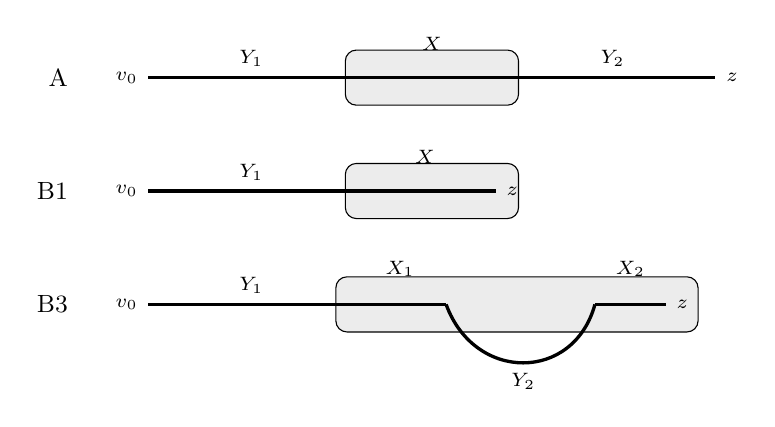
\begin{tikzpicture}[x=0.9cm,y=0.9cm, seg/.style={line width=1.2pt}, xs/.style={draw, rounded corners, fill=gray!15}]
\foreach \row/\lab in {0/A, -1.6/B1, -3.2/B3} { \node[anchor=east] at (-1.0,\row) {\small\lab}; }
% A
\node[xs, minimum width=2.2cm, minimum height=0.7cm] (XA) at (4,0) {};
\draw[seg] (0,0) node[left,font=\scriptsize]{$v_0$} -- (2.9,0) node[midway,above,font=\scriptsize]{$Y_1$};
\draw[seg] (2.9,0) -- (5.1,0) node[midway,above=6pt,font=\scriptsize]{$X$};
\draw[seg] (5.1,0) -- (8,0) node[midway,above,font=\scriptsize]{$Y_2$} node[right,font=\scriptsize]{$z$};
% B1
\node[xs, minimum width=2.2cm, minimum height=0.7cm] at (4,-1.6) {};
\draw[seg] (0,-1.6) node[left,font=\scriptsize]{$v_0$} -- (2.9,-1.6) node[midway,above,font=\scriptsize]{$Y_1$};
\draw[seg] (2.9,-1.6) -- (4.9,-1.6) node[midway,above=6pt,font=\scriptsize]{$X$} node[right,font=\scriptsize]{$z$};
% B3
\node[xs, minimum width=4.6cm, minimum height=0.7cm] at (5.2,-3.2) {};
\draw[seg] (0,-3.2) node[left,font=\scriptsize]{$v_0$} -- (2.9,-3.2) node[midway,above,font=\scriptsize]{$Y_1$};
\draw[seg] (2.9,-3.2) -- (4.2,-3.2) node[midway,above=6pt,font=\scriptsize]{$X_1$};
\draw[seg] (4.2,-3.2) .. controls (4.6,-4.3) and (6.0,-4.3) .. (6.3,-3.2) node[pos=0.5,below,font=\scriptsize]{$Y_2$};
\draw[seg] (6.3,-3.2) -- (7.3,-3.2) node[midway,above=6pt,font=\scriptsize]{$X_2$} node[right,font=\scriptsize]{$z$};
\end{tikzpicture}
\caption{The three types of states relative to a 3-pole $X$ (shaded). Type B3 uses all three cut
edges.}
\label{fig:types}
\end{figure}

\begin{theorem}[Mirror Lemma]\label{thm:mirror}
Under the standing hypothesis, $\pi$ maps every edge of $\cG(G)$ either to an edge of $\cG(H)$ or
to a single vertex. Consequently, the cycle returned on $G$ projects either to the cycle returned
on $H$, or to $C/X$. In the second case it agrees with $C$ outside $X$.
\end{theorem}

\begin{proof}
Let $P \to P'$ be the rotation at the endpoint $z$ of $P$ along $zw$, deleting $ws$. We use
repeatedly that contracting a contiguous block of a sequence commutes with reversing a suffix,
provided the cut point $ws$ is not inside the block.

\emph{Case A ($P$ of type A, $z \in Y_2$).}
\begin{enumerate}
\item[(i)] $w, s \in Y$. The $X$-segment is untouched or reversed as a whole, $P'$ has type A, and
$\pi(P')$ is the rotation of $\pi(P)$ along $zw$.
\item[(ii)] $w \in Y$, $s \in X$. Then $ws$ is the entry cut edge, so $w = q_\inn$ is the last
vertex of $Y_1$ and $s = p_\inn$. Now $P' = Y_1 \cdot \rev(Y_2) \cdot \rev(X)$ has type B1, and
$\pi(P') = Y_1 \cdot \rev(Y_2) \cdot x$ is the rotation of $\pi(P)$ along $zw$, which deletes $wx$.
\item[(iii)] $w \in X$. Then $zw = e_j$ is the unused cut edge, with $z = q_j$ and $w = p_j$. Since
the ports are distinct, $p_j \ne p_\inn, p_{\mathrm{out}}$ is an interior vertex of the
$X$-segment, so $s \in X$. Writing the $X$-segment as $X_a \cdot X_b$ with $X_a$ ending at $w$, we
get $P' = Y_1 \cdot X_a \cdot \rev(Y_2) \cdot \rev(X_b)$, of type B3, with
$\pi(P') = Y_1 \cdot x \cdot \rev(Y_2)$. In $H$, the edge $q_jx$ is not on $\pi(P)$, and the
rotation of $\pi(P)$ along it deletes the edge from $x$ to the first vertex of $Y_2$, giving
exactly $\pi(P')$.
\end{enumerate}

\emph{Case B1 ($P = Y_1 \cdot X$).}
\begin{enumerate}
\item[(i)] $w \in X$. Then $s \in X$, the $Y$-part is unchanged, and $\pi(P') = \pi(P)$.
\item[(ii)] $w \in Y$. Then $z = p_j$ and $w = q_j$ for some $j \ne \inn$. As the $q_i$ are
distinct, $w$ is not the last vertex of $Y_1$, so $s \in Y_1$. Writing $Y_1 = Y_a \cdot Y_b$ with
$Y_a$ ending at $w$, $P' = Y_a \cdot \rev(X) \cdot \rev(Y_b)$ has type A, and
$\pi(P') = Y_a \cdot x \cdot \rev(Y_b)$ is the rotation of $\pi(P) = Y_1 \cdot x$ along $xq_j$. Here
$q_j \ne v_0$ by the standing hypothesis.
\end{enumerate}

\emph{Case B3 ($P = Y_1 \cdot X_1 \cdot Y_2 \cdot X_2$).} All three cut edges are on $P$, so
$w \in X$.
\begin{enumerate}
\item[(i)] $w \in X_2$. Then $s \in X_2$ and $\pi(P') = \pi(P)$.
\item[(ii)] $w \in X_1$, $w \ne p_b$. Then $s \in X_1$. Writing $X_1 = X_{1a} \cdot X_{1b}$ with
$X_{1a}$ ending at $w$, $P' = Y_1 \cdot (X_{1a} \cdot \rev(X_2)) \cdot \rev(Y_2) \cdot \rev(X_{1b})$
has type B3. Its first $X$-piece $X_{1a} \cdot \rev(X_2)$ now ends at the old $p_c$, so the roles
of $p_b$ and $p_c$ are exchanged.
\item[(iii)] $w = p_b$. Then $s = q_b$, and $P' = Y_1 \cdot (X_1 \cdot \rev(X_2)) \cdot \rev(Y_2)$
has type A.
\end{enumerate}
In cases B3(ii) and B3(iii), $\pi(P') = Y_1 \cdot x \cdot \rev(Y_2)$. Since
$\pi(P) = Y_1 \cdot x \cdot Y_2$ ends at $q_c$ and $q_c x$ is not on $\pi(P)$, this is the rotation
of $\pi(P)$ along $q_cx$, which deletes $xq_b$.

No other case occurs, because a non-path edge leads from $Y$ into $X$, or from $X$ into $Y$, only
along an unused cut edge. This proves the first claim.

For the consequence, the walk on $G$ follows the component of $\cG(G)$ from $S_0(G)$ to its other
end $T$. Its image under $\pi$ is a connected subgraph of the component $L$ of $\cG(H)$ that
contains $\pi(S_0(G)) = S_0(H)$ (here $v_{n-1} \in Y$ by the standing hypothesis), and $L$ is a path whose two ends close to $C/X$ and to the cycle
returned on $H$. The endpoint of $T$ is adjacent to $v_0$, so it lies in $Y$ by the standing
hypothesis. Hence $T$ has type A, and $\pi(T)$ is a state of $L$ whose endpoint is adjacent to
$v_0$, i.e.\ an end of $L$. Finally, $\pi(T) = S_0(H)$ means that the cycle closed by $T$ uses
the same edges as $C$ outside $X$.
\end{proof}

\section{Visits and the Transducer Theorem}\label{sec:transducer}

\begin{definition}[visits]
A \emph{visit} to $X$ is a maximal run of consecutive states of the walk whose endpoint lies in
$X$ (states of type B1 or B3), together with the step into the run (its \emph{entry}) and the step
out of it (its \emph{exit}). By the proof of \cref{thm:mirror}, a visit starts from a state of type A whose
$X$-segment is a Hamiltonian path $Q$ of $X$, which we orient from $p_\inn$ to $p_{\mathrm{out}}$.
It has one of two \emph{kinds}:
\begin{description}
\item[B1:] the entry deletes the entry cut edge $e_\inn$ (case A(ii));
\item[B3:] the entry adds the unused cut edge at the third port (case A(iii)).
\end{description}
The \emph{cost} of a B1 visit is the number of steps strictly between its entry and its exit. The
cost of a B3 visit is the number of steps after its entry, up to and including its exit. The
corresponding passage of the walk on $H$ through $x$ takes two steps (B1) or one step (B3), so in
both cases the cost is the number of additional steps caused by $X$. A visit \emph{transmits} if,
after it, the projected walk continues as the walk on $H$ does; otherwise it \emph{reflects}.
\end{definition}

\begin{theorem}[Transducer Theorem]\label{thm:transducer}
For every 3-pole $X$, every oriented Hamiltonian path $Q$ of $X$ between two ports, and every kind
$\kappa \in \{\mathrm{B1}, \mathrm{B3}\}$, there are an outcome (transmit or reflect), a successor
path $Q'$ and a cost $c_X(Q,\kappa)$, such that every visit of kind $\kappa$ that starts with
$X$-segment $Q$, in any host graph satisfying the standing hypothesis, has this outcome, leaves
$X$-segment $Q'$, and has this cost. More strongly, the whole sequence of steps of the visit,
viewed as operations on the $X$-pieces of the state, depends only on $(Q, \kappa)$. Moreover:
\begin{enumerate}
\item outside visits, every step of the walk on $G$ projects to the step that the rule of
\cref{sec:prelim} prescribes on $H$ from the projected state and the corresponding previous
attachment;
\item after a transmitting visit, the walk on $G$ is at a lift of the state reached by the walk on
$H$, with the same previous attachment, where ports are identified with $x$;
\item a reflecting visit ends at a lift of the state from which its entry was made.
\end{enumerate}
\end{theorem}

\begin{proof}
\emph{Independence of the host.} While the endpoint is in $X$, a step is determined by the
endpoint $z$, its neighbours, its predecessor and the previous attachment. In type B1 states every
attachment lies in $X$ and its successor too, so only the $X$-segment changes (case B1(i)), until
the walk leaves along an unused cut edge (case B1(ii)). In type B3 states the steps are of the
forms B3(i), B3(ii), which re-splits the $X$-pieces and reverses $Y_2$ as an opaque block, and the
exit B3(iii). Hence the sequence of $X$-pieces, with their order and orientation, evolves as a
function of $Q$ and $\kappa$ alone. After a B3 entry the previous attachment is the port $p_j$,
which lies in $X$; in a B1 visit it lies in $X$ after the first internal step. At the first step
of a B1 visit it is $q_\inn$, so that visit cannot leave through $p_\inn$ immediately. The cut
edges are part of the data of $X$, and none of them goes to $v_0$, so no other information about
the host enters.

\emph{Item 1.} Outside visits the endpoint $z$ lies in $Y$. The edges at $z$, its predecessor and
the previous attachment correspond in $G$ and $H$ (a port corresponding to $x$). So the admissible
edge corresponds as well, and by cases A(i)--(iii) the step projects to the step of the walk on
$H$.

\emph{Items 2 and 3 for B1.} The entry is the step $S \to S^*$ of the walk on $H$ that makes $x$
the endpoint by deleting $q_\inn x$, after which the previous attachment is $q_\inn$. In $G$ the
state after the entry is $Y_1 \cdot \rev(Y_2) \cdot \rev(Q)$, which ends at $p_\inn$ and whose only
cut edge on the path is $e_{\mathrm{out}}$. (So in the notation of case B1, the entry port of this
B1 state is $p_{\mathrm{out}}$, and the exit is through $p_\inn$ or $p_c$.) The exit
rotates along some cut edge $p_jq_j$ and projects to the rotation of $S^*$ along $xq_j$ (case
B1(ii)), after which the previous attachment is $q_j$ in both graphs. The walk on $H$ continues
from $S^*$ along $xq_c$, where $p_c$ is the third port. So an exit through $p_c$ is that step
(transmit), and an exit through $p_\inn$ is the rotation along $xq_\inn$, which undoes the entry
and returns to $S$ (reflect).

\emph{Items 2 and 3 for B3.} The entry is the step $S \to S^*$ of the walk on $H$ that attaches
$q_j$ to $x$, after which the previous attachment is $x$. Steps of the form B3(ii) project
alternately to $S$ and $S^*$. The exit B3(iii) lands at a lift of $Y_1 \cdot x \cdot \rev(Y_2)$,
which is $S$ or $S^*$, with previous attachment $p_b$, corresponding to $x$. At $S^*$ the walk on
$H$ continues from there (transmit). At $S$ the endpoint $q_j$ has two non-path edges, $q_jx$
(now forbidden) and one other, so the projected walk goes back along $L$ (reflect).

The cost is the number of steps of the visit, which by the first part depends only on $Q$ and
$\kappa$.
\end{proof}

\section{Simple poles}\label{sec:simple}

\begin{lemma}[simple poles transmit]\label{lem:simple}
If $X$ is simple, then every visit to $X$ transmits.
\end{lemma}

\begin{proof}
A state of $H$ of type A (endpoint different from $x$, with $x$ interior) has exactly one lift to
$G$ of type A. Its $Y$-part is determined, and its $X$-segment is the unique Hamiltonian path of
$X$ between the two ports it uses. (If its endpoint is adjacent to $x$, it may also have lifts of
type B3.) Every visit ends in a state of type A, since both kinds of exit, cases B1(ii) and
B3(iii), produce type A. By \cref{thm:transducer}(3), a reflecting visit ends at a lift of the
state from which its entry was made. That state has type A, so the visit ends at its unique
type-A lift, which is the state the walk occupied before the visit. The walk on $G$ would then revisit a state, which is impossible, since it follows
a path in $\cG(G)$.
\end{proof}

\begin{lemma}[composition]\label{lem:composition}
Let $P$ be a 3-pole, and let $X \subset P$ be a simple 3-pole with $N(X) \subseteq P$. Let
$P' = P/X$, with $X$ contracted to a vertex $x$. Then:
\begin{enumerate}
\item[(a)] $h_{ij}(P) = h_{ij}(P')$ for every pair of ports;
\item[(b)] for every visit $(Q, \kappa)$ to $P$ that occurs in some host satisfying the standing
hypothesis, $P$ and $P'$ have the same outcome and successor, under the bijection of (a);
\item[(c)] for every such visit,
\[
c_P(Q,\kappa) \;=\; c_{P'}(Q/X,\kappa) \;+\; \sum_f M_{(Q/X,\kappa),\,f}\; c_X(f),
\]
where $M_{(Q',\kappa), f}$ counts the \emph{passages} of kind $f$ through $x$ during the visit
$(Q',\kappa)$ to $P'$. A passage is a step that makes $x$ the endpoint by deleting $x$'s entry
edge (kind B1), or a step that attaches to $x$ (kind B3), together with the oriented pair of ports
of $X$ that the path uses at that moment.
\end{enumerate}
\end{lemma}

\begin{proof}
(a) The ports of $P$ lie outside $X$: a port of $P$ has a neighbour outside $P$, which would
otherwise lie in $N(X) \setminus P$. So a Hamiltonian path of $P$ between two ports crosses
$\delta(X)$ an even number of times, at most three, and at least once, hence exactly twice. It
therefore consists of a Hamiltonian path of $P'$ together with a Hamiltonian path of $X$ between
the corresponding ports. Since $h_{ij}(X) = 1$, the latter exists and is unique, so this is a
bijection.

(b), (c) Fix a host $G = H_0[y \leftarrow P]$ satisfying the standing hypothesis. Since
$v_0 \notin P \cup N(P)$ and $N(X) \subseteq P$, the standing hypothesis also holds for $X$, and
$G/X = H_0[y \leftarrow P']$. By \cref{lem:simple} and \cref{thm:transducer}, the walk on $G$ is
the walk on $G/X$ in which each passage through $x$ is replaced by a transmitting visit to $X$.
That visit starts in the $X$-segment forced by the simplicity of $X$, and contributes $c_X(f)$
extra steps.

Every passage lies inside a visit to $P'$, possibly sharing its entry or exit. A B3 passage starts
and ends with the endpoint in $N(x) \subseteq P'$. Since $x$ is not a port of $P'$ (by the
argument in (a)), a B1 passage either lies inside a visit, or its step is the entry of the visit;
the latter happens only for an entry of kind B3 that attaches to a port of $P'$ whose successor is
$x$, so that the entry deletes the edge from that port to $x$. Its final step, the rotation at
$x$, may be the exit of the visit, of the form B3(iii). In every case the extra steps lie
strictly inside the window of the corresponding visit to $P$. Therefore visits to $P$ in $G$ and
visits to $P'$ in $G/X$ correspond one-to-one, with the same kind, starting state up to
contraction, outcome and successor, and their costs differ by the inserted costs. The passages
during a visit to $P'$ are determined by the visit (\cref{thm:transducer}), so $M$ does not depend
on the host.
\end{proof}

\begin{remark}
Parts (b) and (c) speak only about visits that occur in some host. If a visit to $P$ occurs in a
host $G$, every passage during it is a visit to $X$ occurring in the same host. In
\cref{sec:proof} we use only visit types that occur, so this is no restriction.
\end{remark}

\section{The construction}\label{sec:construction}

\paragraph{The base graph.} Let $K$ be the cubic graph on $\{0, \dots, 7\}$ consisting of the cycle
$0\,1\,2 \cdots 7\,0$ and the chords $\{0,4\}, \{1,3\}, \{2,6\}, \{5,7\}$ (\cref{fig:K}). It is
3-connected and planar, and has exactly three Hamiltonian cycles. By exhaustive search, it is the
only one of the five connected cubic graphs on 8 vertices with exactly three Hamiltonian cycles. Let $x = 5$ and $r = 2$; then $r \notin N_K[x] = \{4,5,6,7\}$. We
call the neighbours of $r$ the ports $a = 1$, $b = 3$, $c = 6$, and fix the \emph{wiring} that joins
the neighbours $4, 6, 7$ of $x$ to the ports $c, a, b$ of the inner pole, respectively.

\begin{figure}[t]
\centering
\begin{minipage}{0.42\textwidth}\centering
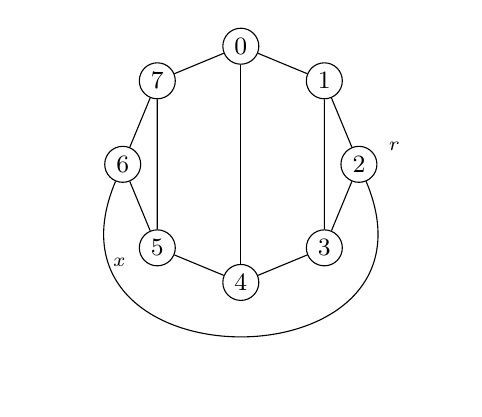
\begin{tikzpicture}[scale=1.5, v/.style={circle, draw, inner sep=1.2pt, minimum size=13pt}]
\foreach \i in {0,...,7} { \node[v] (v\i) at ({90-45*\i}:1) {\small \i}; }
\foreach \i [evaluate=\i as \j using {int(mod(\i+1,8))}] in {0,...,7} { \draw (v\i) -- (v\j); }
\draw (v0) -- (v4); \draw (v1) -- (v3); \draw (v5) -- (v7);
\draw (v2) .. controls (1.8,-1.9) and (-1.8,-1.9) .. (v6);
\node at ($(v5)+(-0.32,-0.12)$) {\scriptsize $x$};
\node at ($(v2)+(0.3,0.15)$) {\scriptsize $r$};
\end{tikzpicture}
\end{minipage}\hfill
\begin{minipage}{0.55\textwidth}\centering
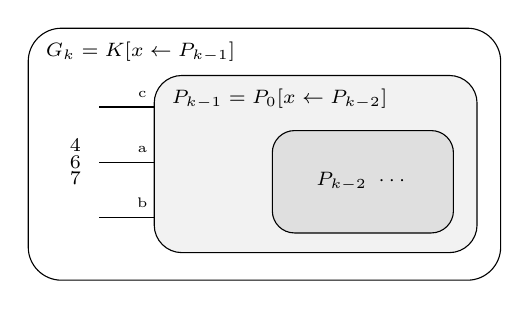
\begin{tikzpicture}[x=1cm,y=1cm]
\draw[rounded corners=12pt] (0,0) rectangle (6,3.2);
\node[anchor=north west,font=\scriptsize] at (0.1,3.15) {$G_k = K[x \leftarrow P_{k-1}]$};
\draw[rounded corners=10pt, fill=gray!10] (1.6,0.35) rectangle (5.7,2.6);
\node[anchor=north west,font=\scriptsize] at (1.7,2.55) {$P_{k-1} = P_0[x \leftarrow P_{k-2}]$};
\draw[rounded corners=8pt, fill=gray!25] (3.1,0.6) rectangle (5.4,1.9);
\node[font=\scriptsize] at (4.25,1.25) {$P_{k-2}\ \cdots$};
\foreach \y/\l in {2.2/c, 1.5/a, 0.8/b} { \draw (0.9,\y) -- (1.6,\y); \node[font=\tiny,above] at (1.45,\y) {\l}; }
\node[font=\scriptsize,align=center] at (0.6,1.5) {$4$\\[-2pt]$6$\\[-2pt]$7$};
\end{tikzpicture}
\end{minipage}
\caption{Left: the base graph $K$, with chords $\{0,4\},\{1,3\},\{5,7\}$ inside and $\{2,6\}$
outside; $x = 5$ is substituted and $r = 2$ deleted. Right: the nesting $G_k = K[x \leftarrow
P_{k-1}]$, where the neighbours $4, 6, 7$ of $x$ are joined to the ports $c, a, b$.}
\label{fig:K}
\end{figure}

\paragraph{The family.} Let $G_0 = K$ and $P_0 = K - r$. For $k \ge 1$ let
$G_k = K[x \leftarrow P_{k-1}]$ with the wiring above, and $P_k = G_k - r$, where $r$ always denotes
the copy of $2$ in the outermost copy of $K$. Then $|V(G_k)| = 8+6k$. Since $r \notin N_K[x]$,
\[
P_k = (K - r)[x \leftarrow P_{k-1}] = P_0[x \leftarrow P_{k-1}]
\qquad\text{and}\qquad
P_k / P_{k-1} = P_0 .
\]
Let $C_k$ be the Hamiltonian cycle of $G_k$ obtained from $0\,1 \cdots 7\,0$ by replacing $x$ with
the unique Hamiltonian path of $P_{k-1}$ between the ports wired to $4$ and $6$. The walk starts at
$v_0 = 0$ with the fixed edge $\{0,1\}$ of the outermost copy.

\begin{lemma}\label{lem:class}
For every $k$, the graph $G_k$ is a 3-connected planar cubic graph with exactly three Hamiltonian
cycles, and $P_k$ is simple.
\end{lemma}

\begin{proof}
\emph{Simplicity and three cycles.} $P_0 = K - r$ is simple. Indeed, each of the three
Hamiltonian cycles of $K$ uses one of the three pairs of edges at $r$; if pair $\{i,j\}$ is used
$m_{ij}$ times, then edge $i$ lies in $m_{ij} + m_{ik}$ cycles, which is even by Smith's theorem
and at most $3$, and the $m$'s sum to $3$. This forces $m_{ij} + m_{ik} = 2$ for every $i$, hence
$m_{ij} = 1$ for every pair, and $h_{ij}(P_0) = m_{ij} = 1$ (also checked in \cref{tab:P0}). If
$P_{k-1}$ is simple, \cref{lem:composition}(a), applied to $P_{k-1} \subset P_k$ with
$P_k / P_{k-1} = P_0$, shows that $P_k$ is simple. A Hamiltonian cycle of
$G_k = K[x \leftarrow P_{k-1}]$ crosses $\delta(P_{k-1})$ exactly twice, so it consists of a
Hamiltonian cycle of $K$, which uses a pair of edges at $x$, together with a Hamiltonian path of
$P_{k-1}$ between the corresponding ports, and this path is unique. Hence $G_k$ has exactly as
many Hamiltonian cycles as $K$, namely three.

\emph{3-connectivity.} For cubic graphs, 3-connectivity is equivalent to 3-edge-connectivity. Let
$G$ and $K$ be 3-edge-connected cubic graphs, $P = G - r$, and suppose $F$ is an edge cut of
$K' = K[x \leftarrow P]$ with $|F| \le 2$ and sides $A, B$. If $V(P)$ lies on one side, contracting
it gives an edge cut of size $|F|$ in $K$, a contradiction. Otherwise let $F_P = F \cap E(P)$.
Placing $r$ on either side of the induced partition of $V(G)$ gives edge cuts of $G$ of sizes
$|F_P|$ plus the number of ports on the other side, and both are at least $3$. Adding the two
inequalities gives $2|F_P| + 3 \ge 6$, so $|F_P| = 2 = |F|$. Then $F \subseteq E(P)$: no wiring
edge and no edge of $K - x$ is in $F$, so each port lies on the same side as its neighbour in $K$.
With $|F_P| = 2$, each of the two inequalities says that the other side contains at least one
port, so both sides contain ports, and hence vertices of $K - x$. Placing $x$ on either side
therefore gives edge cuts of $K$ with both sides nonempty, whose sizes are the numbers of ports on
the other side. Both would have to be at least $3$, which is impossible with three ports.

\emph{Planarity.} Deleting $r$ from a plane embedding of $G_{k-1}$ leaves a face whose boundary
meets the three ports in the cyclic order of the rotation at $r$. Deleting $x$ from a plane
embedding of $K$ leaves a face meeting $N_K(x)$ in the cyclic order of the rotation at $x$. Any
bijection between two 3-element sets either preserves or reverses cyclic order, and a reversal is
undone by mirroring the embedding of $P_{k-1}$. So $P_{k-1}$ can be placed inside that face and
joined to $N_K(x)$ without crossings.
\end{proof}

\section{Proof of the main theorem}\label{sec:proof}

\paragraph{The base gadget.} The pole $P_0 = K - r$ has six oriented pairs of ports, and hence
twelve visit types. \Cref{tab:P0} lists, for each, its cost and its passages through $x$. All
twelve transmit. The passages are named by the ports of the inner pole, through the wiring.
\Cref{app:visits} gives every step.

\begin{table}[t]
\centering\small
\begin{tabular}{lrl}
\toprule
visit & cost & passages through $x$ \\
\midrule
ab/B1 & 3 & ca/B3 \\
ab/B3 & 10 & ab/B1, ac/B1, ac/B3, bc/B1, bc/B3 \\
ac/B1 & 5 & ab/B3, ac/B1 \\
ac/B3 & 10 & ab/B3, ac/B1, ba/B3, bc/B1, cb/B1 \\
ba/B1 & 3 & ca/B1 \\
ba/B3 & 10 & ab/B3, ac/B1, ca/B3, cb/B1 \\
bc/B1 & 5 & ac/B3, bc/B1 \\
bc/B3 & 10 & ab/B1, ac/B3, bc/B1, cb/B3 \\
ca/B1 & 3 & ba/B1 \\
ca/B3 & 6 & ab/B3, ac/B1 \\
cb/B1 & 3 & cb/B3 \\
cb/B3 & 6 & ac/B3, bc/B1 \\
\bottomrule
\end{tabular}
\caption{The twelve visit types of $P_0 = K - r$. The first two letters give the oriented pair of
ports of the visiting path. All visits transmit, and $P_0$ is simple. Together the rows define the
cost vector $c_0$ and the passage matrix $M$.}
\label{tab:P0}
\end{table}

Let $R$ be the set of visit types reachable from ca/B3 in the directed graph of $M$ (defined
below), with an arc $i \to j$ when $M_{ij} > 0$. It consists of the ten types other than ba/B1 and
ca/B1, and it is strongly connected.

\begin{lemma}\label{lem:recursion}
Every type $i \in R$ occurs as a visit to $P_k$, for every $k \ge 0$, in the walk on some $G_m$.
For all $k \ge 1$ and $i \in R$, the visit of type $i$ to $P_k$ transmits with the same successor
as in $P_0$, and
\[
c_k(i) = c_0(i) + \sum_{j} M_{ij}\, c_{k-1}(j),
\]
where only $j \in R$ contribute.
\end{lemma}

\begin{proof}
By \cref{thm:transducer} applied to $X = P_{m-1}$ in $G_m$, the walk on $G_m$ contains a visit of
type ca/B3 to $P_{m-1}$ (see the proof of \cref{thm:main}). If a visit of type $i$ to $P_k$ occurs
in the walk on $G_m$ and $M_{ij} > 0$, then the visit contains a passage of type $j$ through the
copy of $x$ in $P_k$, which is a visit of type $j$ to $P_{k-1}$ in the same walk
(\cref{lem:composition}). By induction on the distance $d$ from ca/B3, a type at distance $d$
occurs as a visit to $P_{m-1-d}$ in $G_m$ for every $m \ge d+1$; taking $m = k+1+d$ gives the
first claim. For the second, apply \cref{lem:composition} to $X = P_{k-1} \subset P = P_k$. This
is allowed since $P_{k-1}$ is simple (\cref{lem:class}), $N(P_{k-1}) = N_K(x) \subseteq P_k$, and
$P_k / P_{k-1} = P_0$. Since $R$ is closed under the arcs of $M$, only $j \in R$ contribute.
\end{proof}

With the visit types ordered ab/B1, ab/B3, ac/B1, ac/B3, ba/B1, ba/B3, bc/B1, bc/B3, ca/B1, ca/B3,
cb/B1, cb/B3, we have $c_0 = (3,10,5,10,3,10,5,10,3,6,3,6)$ and
\[
M = \begin{pmatrix}
0 & 0 & 0 & 0 & 0 & 0 & 0 & 0 & 0 & 1 & 0 & 0 \\
1 & 0 & 1 & 1 & 0 & 0 & 1 & 1 & 0 & 0 & 0 & 0 \\
0 & 1 & 1 & 0 & 0 & 0 & 0 & 0 & 0 & 0 & 0 & 0 \\
0 & 1 & 1 & 0 & 0 & 1 & 1 & 0 & 0 & 0 & 1 & 0 \\
0 & 0 & 0 & 0 & 0 & 0 & 0 & 0 & 1 & 0 & 0 & 0 \\
0 & 1 & 1 & 0 & 0 & 0 & 0 & 0 & 0 & 1 & 1 & 0 \\
0 & 0 & 0 & 1 & 0 & 0 & 1 & 0 & 0 & 0 & 0 & 0 \\
1 & 0 & 0 & 1 & 0 & 0 & 1 & 0 & 0 & 0 & 0 & 1 \\
0 & 0 & 0 & 0 & 1 & 0 & 0 & 0 & 0 & 0 & 0 & 0 \\
0 & 1 & 1 & 0 & 0 & 0 & 0 & 0 & 0 & 0 & 0 & 0 \\
0 & 0 & 0 & 0 & 0 & 0 & 0 & 0 & 0 & 0 & 0 & 1 \\
0 & 0 & 0 & 1 & 0 & 0 & 1 & 0 & 0 & 0 & 0 & 0
\end{pmatrix}.
\]
A direct computation gives the characteristic polynomial
\[
\det(\lambda I - M) = \lambda^2(\lambda-1)^2(\lambda+1)^2(\lambda^2+1)(\lambda^4 - 2\lambda^3 - 2\lambda^2 - 2\lambda - 1).
\]
The quartic factor is irreducible over $\mathbb{Q}$, and its largest real root
$\rho = 2.9477115868\ldots$ is the spectral radius of $M$, and also of its restriction $M_R$ to
$R$. All other eigenvalues of $M$ have modulus at most $1$ (the other roots of the quartic have
moduli $0.584$ and $0.762$).

\begin{proof}[Proof of \cref{thm:main}]
By \cref{lem:class}, $G_k$ is a 3-connected planar cubic graph on $8+6k$ vertices with exactly three
Hamiltonian cycles.

\emph{Exact length.} Apply \cref{thm:transducer} to the 3-pole $X = P_{k-1}$ of $G_k$, so
$H = G_k/X = K$. The standing hypothesis holds, since $0 \notin N_K[x]$. On $K$, the walk from $C$
with fixed edge $\{0,1\}$ takes 4 steps and passes through $x$ once, in a passage of type ca/B3. By
\cref{lem:simple} the corresponding visit transmits, so
\[
\steps(G_k) = 4 + c_{k-1}(\mathrm{ca/B3}).
\]

\emph{Lower bound.} By \cref{lem:recursion}, the vector $c_k$ restricted to $R$ satisfies
$c_k = c_0 + M_R c_{k-1}$ on $R$, where $M_R$ is $M$ restricted to $R$. The integer vector $u$ on
$R$ given in the first column of \cref{tab:cert} satisfies $M_R u \ge \frac{2947}{1000}\,u$
componentwise; this is a finite check. Let $\varepsilon = \min_{i \in R} c_0(i)/u_i > 0$. Since
$c_k \ge M_R c_{k-1}$ on $R$ and $M_R \ge 0$, induction gives
$c_k \ge \varepsilon (2947/1000)^k u$ on $R$. Hence $\steps(G_k) = \Omega(2.947^k)$. The second
column of \cref{tab:cert} is a vector $u'$ with $M_R u' \ge \frac{29477}{10000}\,u'$, which gives
$\Omega(2.9477^k)$ in the same way.

\emph{Sharp lower bound.} Since $R$ is strongly connected, $M_R$ is irreducible, and by the
Perron--Frobenius theorem it has an eigenvector $v > 0$ with $M_R v = \rho(M_R)\, v = \rho v$.
Repeating the argument with $v$ in place of $u$ gives $c_k \ge \varepsilon' \rho^k v$ on $R$, so
$\steps(G_k) = \Omega(\rho^k)$.

\emph{Upper bound.} On $R$, $c_k = \sum_{j=0}^{k} M_R^j c_0$. Since $\rho$ is a simple eigenvalue of
$M_R$ and all others have modulus less than $\rho$, $\|M_R^j\| = O(\rho^j)$, so $c_k = O(\rho^k)$.

Hence $\steps(G_k) = \Theta(\rho^k) = \Theta(\rho^{n/6})$, and $\rho^{1/6} = 1.1974227\ldots$
\end{proof}

\begin{table}[t]
\centering\small
\begin{tabular}{lrr}
\toprule
type & $u$ & $u'$ \\
\midrule
ab/B1 & 77 & 746 \\
ab/B3 & 442 & 4283 \\
ac/B1 & 227 & 2199 \\
ac/B3 & 442 & 4283 \\
ba/B3 & 330 & 3198 \\
bc/B1 & 227 & 2199 \\
bc/B3 & 330 & 3198 \\
ca/B3 & 227 & 2199 \\
cb/B1 & 77 & 746 \\
cb/B3 & 227 & 2199 \\
\bottomrule
\end{tabular}
\caption{Integer vectors with $M_R u \ge 2.947\,u$ and $M_R u' \ge 2.9477\,u'$ componentwise on the
reachable set $R$.}
\label{tab:cert}
\end{table}

\section{Searching the design space}\label{sec:search}

The method gives the exact growth rate of any nested family
$G_k = K[x \leftarrow G_{k-1} - r]$ from the base gadget $K - r$ alone, provided $K - r$ is simple
and $r \notin N_K[x]$. Simplicity forces $K$ to have exactly three Hamiltonian cycles. The growth
rate per vertex is $\rho(M_R)^{1/(|K|-2)}$, where $R$ is the set of visit types reachable from the
passages of the walk on $K$ through $x$.

We enumerated all Hamiltonian cubic graphs with at most 14 vertices, as a Hamiltonian cycle plus a
perfect matching of chords, up to isomorphism. There are 5, 17, 80 and 474 of them on 8, 10, 12
and 14 vertices, in agreement with the known counts. We kept those with exactly three Hamiltonian
cycles: there are 1, 3, 7 and 24 of them. For each, we considered
all choices of $x$, $r \notin N[x]$, wiring, Hamiltonian cycle and start. The best per-vertex rates
are $1.197423$ (8 vertices, our family), $1.184113$ (10), $1.191341$ (12) and $1.197423$ (14). The
best 14-vertex family is two levels of ours. So among nested families of simple poles with the
same gadget at every level and $|K| \le 14$, ours is optimal. Mixing gadgets from level to level, so that $c_k =
c_0^{(k)} + M^{(k)} c_{k-1}$, gives the growth rate of a periodic word as
$\rho(M^{(1)} \cdots M^{(p)})^{1/\sum (|K_i|-2)}$. A beam search over periodic words of length up to
8 over all 1{,}392 distinct gadget matrices with $|K| \le 12$ found nothing better than
$1.197423$. Families whose poles are not simple, so that they may reflect the walk, are outside the
exact theory. Direct simulation of several thousand of them with $|K| \in \{10, 12\}$ gave at most
about $1.189$ per vertex.

\section{Verification}\label{sec:verification}

The computational ingredients of the proof are re-derived by a short standalone script,
\texttt{verify.py}, supplied with this paper. It uses the Python standard library only and runs in
about two seconds. It checks:
\begin{itemize}
\item $K$ has exactly three Hamiltonian cycles, and $P_0$ is simple;
\item all twelve visits of $P_0$ transmit, with the costs and passages of \cref{tab:P0};
\item the reachable set $R$ and both certificates of \cref{tab:cert}, in exact rational
arithmetic;
\item end to end, for $k \le 12$: it builds $G_k$ explicitly, runs Thomason's algorithm from
$(C_k, \{0,1\})$, and compares the number of steps with $4 + c_{k-1}(\mathrm{ca/B3})$, which
reproduces every entry of \cref{tab:steps};
\item for $k \le 3$: cubic, exactly three Hamiltonian cycles (by exhaustive search), and
3-edge-connected.
\end{itemize}
The remaining computational claims are not needed for \cref{thm:main} and are checked by separate
scripts: the search of \cref{sec:search}, with exact isomorphism tests (which also shows that $K$
is the only cubic graph on 8 vertices with exactly three Hamiltonian cycles), and the direct checks
of the graph class for larger $n$ reported below.
We also tested the ingredients independently of this script. An edge-set implementation of the
algorithm and a brute-force traversal of the full state graph agree with it on all tested graphs.
The Mirror Lemma and the Transducer Theorem were checked on thousands of random hosts and 3-poles.
\Cref{lem:composition} was checked on $71{,}484$ random pairs $(P', X)$, and \cref{lem:simple} on
$7{,}233$ random simple poles with up to 21 vertices, without exception. When $X$ is not simple, the
conclusions of \cref{lem:composition} fail in most cases, so the hypothesis cannot be dropped.
Planarity, 3-connectivity and the number of Hamiltonian cycles were confirmed directly for
$n \le 80$, $n \le 68$ and $n \le 50$, respectively.

\section{Discussion and open problems}\label{sec:discussion}

The Mirror Lemma and the Transducer Theorem show that a 3-edge cut behaves like a reversible
finite-state gadget that passes the walk through or reflects it. The lollipop walk is then a
deterministic reversible particle moving through such gadgets, which is the setting of zero-player
reversible motion planning, where PSPACE-hardness results are known~\cite{DHHL22}. Simple poles
never reflect, so they cannot carry information by themselves. Poles with several internal paths
can reflect, and their state persists between visits. We believe this is a possible route to
Eppstein's question~\cite{Eppstein23} whether computing the output of the lollipop algorithm is
FP$^{\textsf{PSPACE}}$-complete.

\begin{itemize}
\item Is there an exact composition theory for non-simple poles, and do such poles give larger
bases?
\item Does the method extend to 4-edge cuts? This would be needed for cyclically 4-edge-connected
graphs, the class of Zhong's examples and of Thomassen's reduction.
\item Is there an upper bound of the form $c^n$ with $c < 2$ on the length of the lollipop walk in
cubic graphs?
\item Is the lollipop walk polynomial on cyclically 5-edge-connected cubic graphs?
\end{itemize}

\paragraph{Acknowledgements.} ACKNOWLEDGEMENTS. [If required by the venue: a statement on the use
of AI assistance.]

\begin{thebibliography}{99}
\bibitem{Tutte46} W.\,T.~Tutte. On Hamiltonian circuits. \emph{J. London Math. Soc.} 21 (1946),
98--101.
\bibitem{Thomason78} A.\,G.~Thomason. Hamiltonian cycles and uniquely edge colourable graphs.
\emph{Ann. Discrete Math.} 3 (1978), 259--268.
\bibitem{Papadimitriou94} C.\,H.~Papadimitriou. On the complexity of the parity argument and other
inefficient proofs of existence. \emph{J. Comput. System Sci.} 48(3) (1994), 498--532.
\bibitem{Krawczyk99} A.~Krawczyk. The complexity of finding a second Hamiltonian cycle in cubic
graphs. \emph{J. Comput. System Sci.} 58(3) (1999), 641--647.
\bibitem{Cameron01} K.~Cameron. Thomason's algorithm for finding a second hamiltonian circuit
through a given edge in a cubic graph is exponential on Krawczyk's graphs. \emph{Discrete Math.}
235 (2001), 69--77.
\bibitem{Zhong18} L.~Zhong. The complexity of Thomason's algorithm for finding a second Hamiltonian
cycle. \emph{Bull. Aust. Math. Soc.} 98(1) (2018), 18--26.
\bibitem{IML15} Problem collection from the IML programme: Graphs, Hypergraphs, and Computing.
arXiv:1511.00270 (2015).
\bibitem{BrianskiSzady22} M.~Bria\'nski and A.~Szady. A short note on graphs with long Thomason
chains. \emph{Discrete Math.} 345(1) (2022), 112624. arXiv:1903.02515.
\bibitem{BKN24} A.~Bj\"orklund, P.~Kaski and J.~Nederlof. Another Hamiltonian cycle in bipartite
Pfaffian graphs. In \emph{ICALP 2024}, LIPIcs 297, 26. arXiv:2308.01574.
\bibitem{DMSZ20} A.~Deligkas, G.\,B.~Mertzios, P.\,G.~Spirakis and V.~Zamaraev. Exact and
approximate algorithms for computing a second Hamiltonian cycle. In \emph{MFCS 2020}, LIPIcs 170,
27. arXiv:2004.06036.
\bibitem{Eppstein23} D.~Eppstein. The complexity of iterated reversible computation.
\emph{TheoretiCS} 2 (2023), Article 10. arXiv:2112.11607.
\bibitem{DHHL22} E.\,D.~Demaine, R.\,A.~Hearn, D.~Hendrickson and J.~Lynch. PSPACE-completeness of
reversible deterministic systems. In \emph{Machines, Computations, and Universality (MCU 2022)},
LNCS 13419, Springer (2022), 91--108. arXiv:2207.07229.
\end{thebibliography}

\appendix
\section{Every step of the twelve visits of \texorpdfstring{$P_0$}{P0}}\label{app:visits}

Vertices carry their labels in $K$. The column $Q$ lists the internal path of the visit, from the
port nearer $v_0$. A B1 visit starts with the endpoint at the first vertex of $Q$, with $Q$
reversed. A B3 visit starts after the cut edge at the third port has been added; the internal path
is then split after that port. Each step $zw$ rotates at the endpoint $z$ along the edge $zw$.
${}^{\dagger}$ marks a step that makes $x = 5$ the endpoint (a B1 passage), and ${}^{\ddagger}$ a
step that attaches to $x$ (a B3 passage). A ${}^{\dagger}$ on the visit name means that its entry
is itself a B1 passage. Every visit transmits.

{\small
\begin{longtable}{@{}l l >{\raggedright\arraybackslash}p{6.4cm} r >{\raggedright\arraybackslash}p{3.6cm}@{}}
\toprule
visit & $Q$ & steps after the entry & cost & passages through $x$ \\
\midrule
\endhead
ab/B1 & 1076543 & $13$ $40$ $75^{\ddagger}$ & 3 & ca/B3 \\
ab/B3$^{\dagger}$ & 1076543 & $57$ $65^{\ddagger}$ $40$ $76^{\dagger}$ $54$ $31$ $07^{\dagger}$ $56$ $75^{\ddagger}$ $43$ & 10 & ab/B1, ac/B1, ac/B3, bc/B1, bc/B3 \\
ac/B1 & 1340756 & $10$ $45^{\ddagger}$ $76^{\dagger}$ $57$ $04$ & 5 & ab/B3, ac/B1 \\
ac/B3 & 1340756 & $45^{\ddagger}$ $76^{\dagger}$ $57$ $01$ $34^{\dagger}$ $56$ $70$ $45^{\ddagger}$ $67^{\dagger}$ $56$ & 10 & ab/B3, ac/B1, ba/B3, bc/B1, cb/B1 \\
ba/B1 & 3456701 & $31$ $04^{\dagger}$ $57$ & 3 & ca/B1 \\
ba/B3 & 3456701 & $75^{\ddagger}$ $67$ $04^{\dagger}$ $56$ $70$ $13$ $45^{\ddagger}$ $76^{\dagger}$ $57$ $01$ & 10 & ab/B3, ac/B1, ca/B3, cb/B1 \\
bc/B1 & 3104576 & $34$ $07^{\dagger}$ $56$ $75^{\ddagger}$ $40$ & 5 & ac/B3, bc/B1 \\
bc/B3 & 3104576 & $07^{\dagger}$ $56$ $75^{\ddagger}$ $43$ $10$ $76^{\dagger}$ $54$ $07$ $65^{\ddagger}$ $76$ & 10 & ab/B1, ac/B3, bc/B1, cb/B3 \\
ca/B1 & 6570431 & $67^{\dagger}$ $54$ $01$ & 3 & ba/B1 \\
ca/B3 & 6570431 & $10$ $45^{\ddagger}$ $76^{\dagger}$ $57$ $04$ $31$ & 6 & ab/B3, ac/B1 \\
cb/B1 & 6754013 & $65^{\ddagger}$ $70$ $43$ & 3 & cb/B3 \\
cb/B3 & 6754013 & $34$ $07^{\dagger}$ $56$ $75^{\ddagger}$ $40$ $13$ & 6 & ac/B3, bc/B1 \\
\bottomrule
\end{longtable}
}

\section{A worked example: the walk on \texorpdfstring{$G_1$}{G1}}\label{app:example}

$G_1 = K[x \leftarrow P_0]$ has 14 vertices. Outer vertices are written $0, \dots, 7$ (without $5$),
and the inner copy of $K - r$ as $0', 1', 3', \dots, 7'$. The wiring joins $4$--$6'$, $6$--$1'$ and
$7$--$3'$. The walk starts from $C_1$ with fixed edge $\{0,1\}$. Steps marked $\bullet$ have their
endpoint inside the inner pole. Step 1 is the entry of a B3 visit of type ca/B3, and steps 2--7 are
its cost $c_0(\mathrm{ca/B3}) = 6$, ending at step 7. The total is $4 + 6 = 10$ steps, as predicted.

{\small
\begin{longtable}{@{}r l c l@{}}
\toprule
step & rotation $(z,w)$ & & path after the step \\
\midrule
\endhead
0 & -- &  & 0 1 2 3 4 6$'$ 5$'$ 7$'$ 0$'$ 4$'$ 3$'$ 1$'$ 6 7 \\
1 & (7,3$'$) & $\bullet$ & 0 1 2 3 4 6$'$ 5$'$ 7$'$ 0$'$ 4$'$ 3$'$ 7 6 1$'$ \\
2 & (1$'$,0$'$) & $\bullet$ & 0 1 2 3 4 6$'$ 5$'$ 7$'$ 0$'$ 1$'$ 6 7 3$'$ 4$'$ \\
3 & (4$'$,5$'$) & $\bullet$ & 0 1 2 3 4 6$'$ 5$'$ 4$'$ 3$'$ 7 6 1$'$ 0$'$ 7$'$ \\
4 & (7$'$,6$'$) & $\bullet$ & 0 1 2 3 4 6$'$ 7$'$ 0$'$ 1$'$ 6 7 3$'$ 4$'$ 5$'$ \\
5 & (5$'$,7$'$) & $\bullet$ & 0 1 2 3 4 6$'$ 7$'$ 5$'$ 4$'$ 3$'$ 7 6 1$'$ 0$'$ \\
6 & (0$'$,4$'$) & $\bullet$ & 0 1 2 3 4 6$'$ 7$'$ 5$'$ 4$'$ 0$'$ 1$'$ 6 7 3$'$ \\
7 & (3$'$,1$'$) &  & 0 1 2 3 4 6$'$ 7$'$ 5$'$ 4$'$ 0$'$ 1$'$ 3$'$ 7 6 \\
8 & (6,2) &  & 0 1 2 6 7 3$'$ 1$'$ 0$'$ 4$'$ 5$'$ 7$'$ 6$'$ 4 3 \\
9 & (3,1) &  & 0 1 3 4 6$'$ 7$'$ 5$'$ 4$'$ 0$'$ 1$'$ 3$'$ 7 6 2 \\
10 & (2,3) &  & 0 1 3 2 6 7 3$'$ 1$'$ 0$'$ 4$'$ 5$'$ 7$'$ 6$'$ 4 \\
\bottomrule
\end{longtable}
}

\end{document}
